\documentclass[11pt,a4paper]{article}
\usepackage[utf8]{inputenc}
\usepackage[T1]{fontenc}
\usepackage{lmodern}
\usepackage[brazilian]{babel}
\usepackage[margin=2.2cm]{geometry}
\usepackage{amsmath,amssymb}
\usepackage{graphicx}
\usepackage{booktabs}
\usepackage{float}
\usepackage{caption}
\usepackage{hyperref}
\usepackage{enumitem}
\setlist{nosep}
\captionsetup{font=small}

\title{Trabalho Prático: Divisão e Conquista\\\large Projeto e Análise de Algoritmos}
\author{Amanda Uchoa \and [nome do(a) colega]}
\date{Universidade de Fortaleza (UNIFOR), 2026}

\begin{document}
\renewcommand{\tablename}{Tabela}
\renewcommand{\figurename}{Figura}
\maketitle

\section{Introdução}

Este relatório apresenta a implementação e a análise de dois problemas resolvidos com divisão e conquista (D\&C): o \emph{subarranjo de soma máxima} (Etapa~1) e o \emph{par de pontos mais próximos} (Etapa~2). Cada um foi comparado com uma solução de força bruta e, na Etapa~1, também com a versão $O(n)$ (Kadane). Todo o código está em Python~3, no repositório junto com as instruções de execução (\texttt{README.md}), os casos de teste (\texttt{casos\_de\_teste.json}) e as medições brutas (\texttt{resultados/medicoes.csv}).

Os algoritmos de ordenação vistos em aula (merge sort e quick sort) foram reaproveitados na Etapa~2. O \emph{quick sort} faz a ordenação inicial por $x$, e a função \texttt{combinacao} do \emph{merge sort} mantém os pontos ordenados por $y$ durante a recursão. Duas mudanças foram necessárias. A versão da aula da \texttt{combinacao} não incrementava \texttt{i} e entrava em laço infinito, e isso foi corrigido. O quick sort passou a sortear o pivô, porque com o pivô fixo no fim um vetor já ordenado cai no pior caso $O(n^2)$ e estoura o limite de recursão do Python.

\section{Etapa 1: Subarranjo de Soma Máxima}

\paragraph{Entrada e saída.} A entrada é $n$ seguido de $n$ inteiros. A saída é a soma máxima e os índices (a partir de 0) de início e fim. O intervalo tem pelo menos um elemento, então um vetor só de negativos devolve o maior negativo. \textbf{Regra de desempate:} maior soma; se empatar, menor início; se empatar de novo, menor fim. As três implementações seguem a mesma regra, e os testes aleatórios conferem que elas devolvem exatamente a mesma tripla.

\paragraph{Força bruta.} Para cada início $i$, o laço interno avança o fim $j$ e reaproveita a soma anterior (\texttt{soma += v[j]}). O número de intervalos testados é
$\sum_{i=0}^{n-1}(n-i) = \frac{n(n+1)}{2} = \Theta(n^2)$.
A melhor resposta só é trocada quando a soma é \emph{estritamente} maior, e isso já garante o menor $i$ e o menor $j$.

\paragraph{Divisão e conquista.} O vetor é dividido ao meio, como no merge sort, e cada metade é resolvida recursivamente. Depois, em $O(n)$, calcula-se o melhor subarranjo que \emph{cruza o meio}: anda-se do meio para a esquerda guardando a melhor soma (com \texttt{>=}, para ficar com o início mais à esquerda nos empates) e do meio$+1$ para a direita (com \texttt{>}, para ficar com o fim mais à esquerda). A resposta é o melhor dos três candidatos. Todo subarranjo está inteiro na esquerda, inteiro na direita ou cruza o meio, e cada candidato já é o melhor de sua categoria pela regra de desempate. Por isso a combinação está correta. A recorrência é
\[
T(n) = 2\,T(n/2) + \Theta(n), \qquad T(1)=\Theta(1).
\]
Pelo Teorema Mestre ($a=2$, $b=2$, $f(n)=\Theta(n)=\Theta(n^{\log_2 2})$, caso~2), $T(n)=\Theta(n\log n)$. Na árvore de recursão, cada um dos $\log_2 n$ níveis custa $cn$ no total, o que dá o mesmo resultado.

\paragraph{Questão desafio: Kadane, $O(n)$.} Seja $M_j$ a melhor soma de um intervalo que \emph{termina} em $j$. Vale $M_j = \max(v_j,\; M_{j-1}+v_j)$: o intervalo continua se $M_{j-1}\ge 0$ e recomeça em $j$ se $M_{j-1}<0$. Usar $\ge$ em vez de $>$ faz com que, quando $M_{j-1}=0$, o intervalo continue. A soma é a mesma, mas o início é menor, como pede a regra. A resposta é o melhor $M_j$, com um único laço: $T(n)=\Theta(n)$.

\section{Etapa 2: Par de Pontos Mais Próximos}

\paragraph{Força bruta.} Compara os $\binom{n}{2}=\Theta(n^2)$ pares.

\paragraph{Divisão e conquista.}
\begin{enumerate}
  \item Ordenação inicial por $x$ (desempate por $y$) com o quick sort de pivô aleatório: $O(n\log n)$ esperado.
  \item Divisão na mediana: os $\lfloor n/2\rfloor$ primeiros vão para a esquerda e o resto para a direita. A linha vertical fica em $x_m = x$ do ponto do meio. Dividir pela \emph{posição} na lista ordenada, e não pelo valor de $x$, garante metades de tamanho equilibrado mesmo quando muitos pontos têm o mesmo $x$ (caso de teste E2-03).
  \item Cada lado é resolvido recursivamente e $\delta=\min(\delta_E,\delta_D)$. Cada chamada também devolve seus pontos \emph{ordenados por $y$}, e as duas listas são juntadas pela \texttt{combinacao} do merge sort em $O(n)$.
  \item Monta-se a faixa $\{p : |p_x-x_m|<\delta\}$, já ordenada por $y$. Cada ponto é comparado com \textbf{no máximo os 7 seguintes} da faixa, parando antes se a diferença em $y$ já for $\ge\delta$.
  \item \textbf{Limiar:} se o subproblema tem até $L$ pontos, ele é resolvido por força bruta. Escolhemos $L=8$ (Seção~\ref{sec:limiar}).
\end{enumerate}
O passo 3 evita ordenar por $y$ em cada nível, o que daria $\Theta(n\log^2 n)$. Com ele, dividir (fatiar a lista), juntar por $y$ e varrer a faixa custam $O(n)$ por chamada:
\[
T(n) = 2\,T(n/2) + \Theta(n), \qquad T(n)=\Theta(L^2)\ \text{se } n\le L.
\]
A árvore tem $\log_2(n/L)$ níveis de custo $cn$ e $n/L$ folhas de custo $\Theta(L^2)$. Logo $T(n)=\Theta\!\left(n\log\frac{n}{L} + nL\right)=\Theta(n\log n)$ para $L$ constante, e somando a ordenação inicial o total continua $\Theta(n\log n)$.

\paragraph{Por que bastam 7 comparações por ponto na faixa.} Seja $p$ um ponto da faixa e considere os pontos que vêm \emph{depois} dele na ordem por $y$ e que podem estar a menos de $\delta$ de $p$. Todos estão no retângulo $R=[x_m-\delta,\,x_m+\delta]\times[p_y,\,p_y+\delta]$, de tamanho $2\delta\times\delta$. Divida $R$ em dois quadrados $\delta\times\delta$, um de cada lado da linha. Os pontos da metade esquerda estão todos a uma distância $\ge\delta_E\ge\delta$ uns dos outros. Em um quadrado $\delta\times\delta$ cabem no máximo 4 pontos com essa propriedade: dividindo o quadrado em 4 quadradinhos $\frac{\delta}{2}\times\frac{\delta}{2}$, dois pontos no mesmo quadradinho estariam a no máximo $\frac{\delta}{\sqrt2}<\delta$, o que é uma contradição. O mesmo vale para a direita. Assim, $R$ tem no máximo $4+4=8$ pontos, incluindo o próprio $p$, e por isso só é preciso olhar \textbf{os 7 seguintes}. Pontos em cima da linha pertencem a um lado só (o da sua posição na lista), então a contagem continua valendo com coordenadas $x$ repetidas. Como a varredura é feita para todo $p$, cada par próximo é encontrado a partir do ponto de menor posição na ordem por $y$.

\section{Testes}

A bateria (\texttt{testes.py}, 15 testes do \texttt{unittest}, todos passando) tem três partes:
\begin{enumerate}
  \item \textbf{Casos fixos} (\texttt{casos\_de\_teste.json}): 18 da Etapa~1 e 12 da Etapa~2, cada um com entrada, saída esperada e \textbf{justificativa} escrita no próprio arquivo. Os casos da Etapa~2 rodam a D\&C com os limiares 1, 2, 3, 4, 8, 12 e 16. Com limiares pequenos, mesmo entradas pequenas passam pela recursão e pela faixa.
  \item \textbf{Testes aleatórios contra a força bruta}: 3000 vetores na Etapa~1 (valores em faixas pequenas como $[-2,2]$, que geram muitos empates) e 1800 conjuntos de pontos na Etapa~2 (inteiros em grades pequenas, que geram pontos repetidos e $x$ iguais, e também reais). Também verificamos se a soma devolvida é de fato a soma do intervalo devolvido e se o par devolvido realmente tem a distância informada.
  \item \textbf{Linha de comando}: os scripts são executados com a entrada pelo \texttt{stdin}, como o professor fará.
\end{enumerate}

\begin{table}[H]\centering\small
\begin{tabular}{p{2.1cm}p{12.6cm}}
\toprule
Casos & Motivo \\ \midrule
E1-01 a 03 & \textbf{Tamanho 1} (positivo, negativo e zero): é o caso base da recursão. \\
E1-04, 05, 18 & \textbf{Só negativos}: a resposta é o maior negativo. Uma implementação que começa com \texttt{melhor = 0} erra aqui. \\
E1-08 a 11 & \textbf{Empates}: intervalos disjuntos, intervalos encaixados, zeros e vetor todo de zeros. O E1-10 ($[0,0,5,0]\to(5,0,2)$) testa se o Kadane continua o intervalo quando a soma atual é 0. \\
E1-12 a 15 & Resposta cruzando o meio, só na metade direita, só na esquerda, e atravessando um negativo. \\
E1-16 & Soma maior que $2^{31}$: em Python não há estouro, mas em C/Java haveria. \\
E2-01 & $n=2$, a menor entrada válida. \\
E2-02 & \textbf{Pontos repetidos}: $\delta=0$ e a faixa fica vazia. \\
E2-03, 04 & Todos com o mesmo $x$ (a linha passa em cima de todos) ou o mesmo $y$. \\
E2-05, 11 & Par mais próximo com um ponto de cada lado da linha: só é achado na faixa. \\
E2-06, 07, 12 & Coordenadas negativas, reais e grandes. \\
E2-08, 09 & Empates de distância e grade $3\times3$ (muitos pontos dentro da faixa). \\
\bottomrule
\end{tabular}
\caption{Casos de borda e por que foram incluídos (o texto completo está no JSON).}
\end{table}

\section{Etapa 3: Análise Experimental}

\paragraph{Metodologia.} Para cada $n\in\{100,200,400,800,1600,3200,6400\}$ foram feitas \textbf{5 execuções}, cada uma com uma entrada aleatória nova: inteiros em $[-100,100]$ na Etapa~1 e pontos reais em $[0,10^4]^2$ na Etapa~2. O tempo foi medido com \texttt{time.perf\_counter} e o coletor de lixo desligado durante a medição. As tabelas mostram média $\pm$ desvio padrão. Para entradas pequenas ($n\le 256$), cada execução repete a chamada várias vezes e divide o tempo, porque uma chamada sozinha é rápida demais para o relógio. \textbf{Máquina:} Intel Xeon @ 2,10\,GHz (2 núcleos, máquina virtual em nuvem), 7,8\,GB de RAM, Linux 6.18, Python 3.13.18. Por ser uma VM compartilhada, há algum ruído, visível nos desvios padrão.

\begin{table}[H]\centering\small
\begin{tabular}{rrrr}
\hline
$n$ & Forca bruta (ms) & Divisao e conquista (ms) & Kadane O(n) (ms) \\
\hline
100 & 0.250 $\pm$ 0.035 & 0.112 $\pm$ 0.005 & 0.028 $\pm$ 0.012 \\
200 & 0.976 $\pm$ 0.137 & 0.235 $\pm$ 0.014 & 0.035 $\pm$ 0.005 \\
400 & 3.585 $\pm$ 0.044 & 0.506 $\pm$ 0.013 & 0.068 $\pm$ 0.007 \\
800 & 14.983 $\pm$ 0.184 & 0.999 $\pm$ 0.020 & 0.121 $\pm$ 0.007 \\
1600 & 62.275 $\pm$ 1.928 & 2.172 $\pm$ 0.201 & 0.226 $\pm$ 0.019 \\
3200 & 258.692 $\pm$ 16.899 & 4.878 $\pm$ 1.206 & 0.494 $\pm$ 0.123 \\
6400 & 1085.848 $\pm$ 52.383 & 8.867 $\pm$ 0.226 & 0.976 $\pm$ 0.060 \\
\hline
\end{tabular}

\caption{Etapa 1: tempo médio em milissegundos (5 execuções).}\label{tab:e1}
\end{table}

\begin{table}[H]\centering\small
\begin{tabular}{rrr}
\hline
$n$ & Forca bruta (ms) & Divisao e conquista (ms) \\
\hline
100 & 0.705 $\pm$ 0.029 & 0.389 $\pm$ 0.037 \\
200 & 2.842 $\pm$ 0.046 & 0.802 $\pm$ 0.049 \\
400 & 12.345 $\pm$ 1.175 & 1.663 $\pm$ 0.028 \\
800 & 46.615 $\pm$ 0.216 & 3.668 $\pm$ 0.070 \\
1600 & 197.011 $\pm$ 13.338 & 7.879 $\pm$ 0.312 \\
3200 & 785.315 $\pm$ 47.873 & 17.384 $\pm$ 1.490 \\
6400 & 3156.367 $\pm$ 39.157 & 39.603 $\pm$ 3.453 \\
\hline
\end{tabular}

\caption{Etapa 2: tempo médio em milissegundos (5 execuções, D\&C com limiar 8).}\label{tab:e2}
\end{table}

\begin{figure}[H]\centering
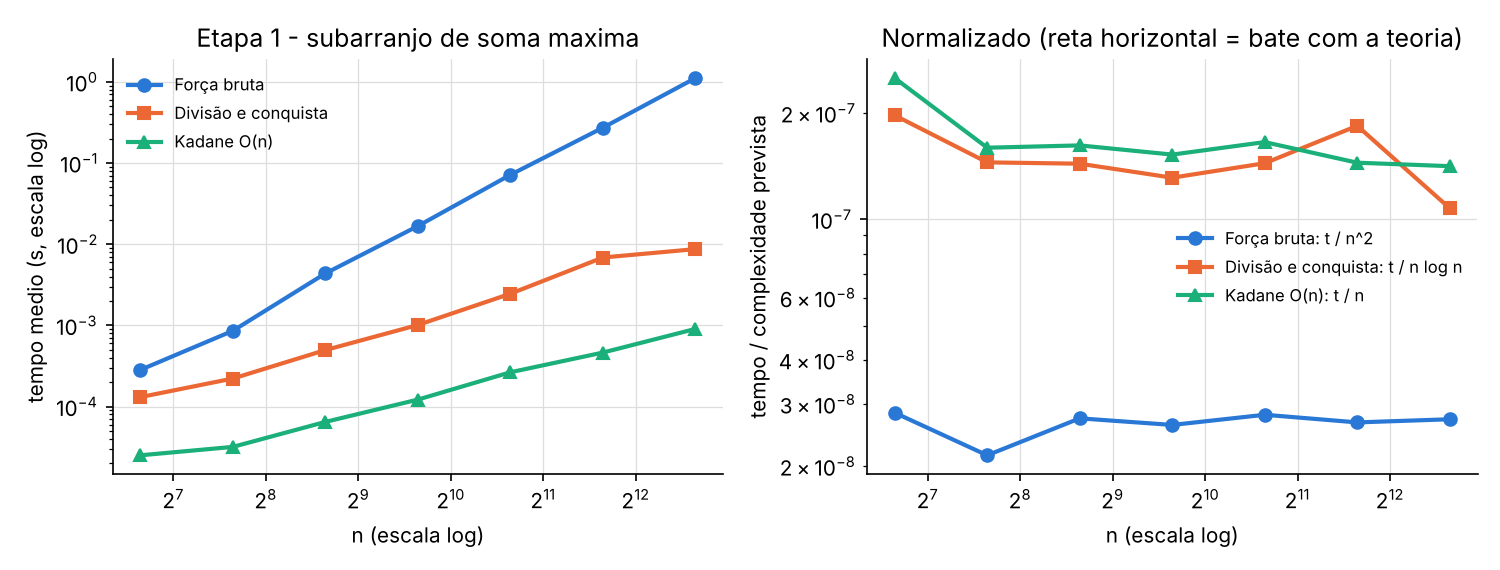
\includegraphics[width=\linewidth]{../resultados/etapa1_tempos.png}
\caption{Etapa 1. À esquerda, os tempos (log-log). À direita, o tempo dividido pela complexidade prevista: uma curva horizontal significa que o crescimento bate com a análise.}\label{fig:e1}
\end{figure}

\begin{figure}[H]\centering
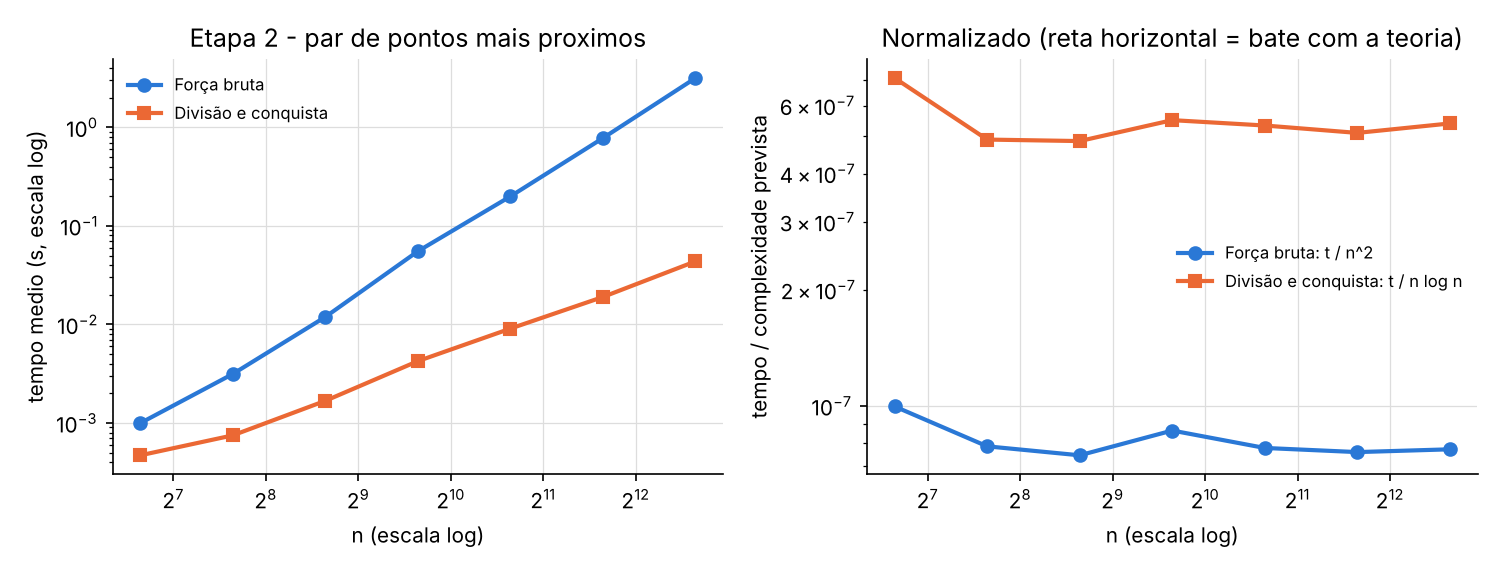
\includegraphics[width=\linewidth]{../resultados/etapa2_tempos.png}
\caption{Etapa 2, com as mesmas convenções da Figura~\ref{fig:e1}.}\label{fig:e2}
\end{figure}

\subsection{Comparação com a análise teórica}

Em um gráfico log-log, $t=c\,n^k$ vira uma reta de inclinação $k$. Também é útil olhar quanto o tempo cresce quando $n$ dobra: para $n^2$ o fator esperado é 4, e para $n\log n$, com $n$ grande, é um pouco mais de 2 (de 3200 para 6400 o fator é $2\cdot\frac{12{,}64}{11{,}64}\approx 2{,}17$).

\begin{itemize}
  \item \textbf{Força bruta (as duas etapas).} Os gráficos mostram retas de inclinação 2, e as curvas normalizadas $t/n^2$ são praticamente horizontais. Na Etapa~1, de 3200 para 6400 o tempo foi multiplicado por $1111{,}8/272{,}3\approx4{,}1$. Na Etapa~2, de 1600 para 6400 (fator teórico 16) o tempo foi multiplicado por $3164/199{,}4\approx15{,}9$. Isso confirma o $\Theta(n^2)$.
  \item \textbf{D\&C da Etapa 2.} A curva $t/(n\log n)$ fica quase horizontal a partir de $n\approx400$. De 1600 para 6400 o tempo cresceu $43{,}6/9{,}07\approx4{,}8$ vezes, contra os $4\cdot\frac{12{,}64}{10{,}64}\approx4{,}75$ previstos para $n\log n$. A concordância é muito boa.
  \item \textbf{D\&C da Etapa 1.} A curva $t/(n\log n)$ cai devagar (de $\approx2{,}0\cdot10^{-7}$ para $\approx1{,}1\cdot10^{-7}$). Isso acontece porque o custo real é $c_1 n\log n + c_2 n$: a recursão faz cerca de $2n$ chamadas de função, e em Python cada chamada (com a criação das tuplas de resposta) custa caro. O termo $c_2 n$ pesa relativamente mais nos $n$ pequenos. (O ponto de $n=3200$ fica fora da tendência por ruído da máquina virtual: o desvio padrão dele foi de 50\% da média.) A complexidade assintótica continua $\Theta(n\log n)$, e o termo de ordem menor só aparece porque a faixa de $n$ medida é pequena.
  \item \textbf{Kadane.} A curva $t/n$ é horizontal a partir de $n=200$, confirmando $\Theta(n)$. O primeiro ponto ($n=100$, $\approx25\,\mu$s) está acima porque, nessa escala, o custo fixo da chamada e da medição domina.
\end{itemize}

\subsection{Quando a força bruta vence e quando a técnica vence}

\begin{table}[H]\centering\small
\begin{tabular}{rrrr}
\hline
$n$ & Forca bruta ($\mu$s) & Divisao e conquista ($\mu$s) & Kadane O(n) ($\mu$s) \\
\hline
2 & 0.393 $\pm$ 0.015 & 0.720 $\pm$ 0.052 & 0.275 $\pm$ 0.009 \\
4 & 0.750 $\pm$ 0.038 & 1.836 $\pm$ 0.055 & 0.463 $\pm$ 0.015 \\
8 & 1.962 $\pm$ 0.087 & 4.432 $\pm$ 0.048 & 0.924 $\pm$ 0.035 \\
16 & 6.354 $\pm$ 0.129 & 10.074 $\pm$ 0.053 & 1.914 $\pm$ 0.138 \\
32 & 22.405 $\pm$ 0.507 & 22.359 $\pm$ 0.293 & 3.848 $\pm$ 0.076 \\
64 & 87.876 $\pm$ 4.765 & 48.977 $\pm$ 0.853 & 7.598 $\pm$ 0.376 \\
128 & 342.785 $\pm$ 12.898 & 105.642 $\pm$ 1.888 & 15.979 $\pm$ 0.444 \\
256 & 1389.513 $\pm$ 66.037 & 247.125 $\pm$ 15.190 & 35.678 $\pm$ 8.118 \\
\hline
\end{tabular}
\\[6pt]
\begin{tabular}{rrr}
\hline
$n$ & Força bruta ($\mu$s) & Divisão e conquista ($\mu$s) \\
\hline
2 & 0.445 $\pm$ 0.026 & 2.273 $\pm$ 0.036 \\
4 & 1.328 $\pm$ 0.101 & 6.394 $\pm$ 0.288 \\
8 & 5.084 $\pm$ 0.403 & 16.485 $\pm$ 0.793 \\
16 & 18.035 $\pm$ 0.284 & 41.918 $\pm$ 3.997 \\
32 & 71.052 $\pm$ 1.412 & 94.132 $\pm$ 4.938 \\
64 & 280.757 $\pm$ 4.400 & 205.899 $\pm$ 3.373 \\
128 & 1191.766 $\pm$ 130.965 & 498.194 $\pm$ 76.730 \\
256 & 5082.719 $\pm$ 601.443 & 1182.133 $\pm$ 222.154 \\
\hline
\end{tabular}

\caption{Entradas pequenas, em microssegundos. Em cima, a Etapa 1; embaixo, a Etapa 2 (D\&C ``pura'', com limiar 3).}\label{tab:peq}
\end{table}

A complexidade assintótica só diz qual algoritmo vence \emph{para $n$ suficientemente grande}. Para $n$ pequeno, o que decide são as constantes. A força bruta tem um laço muito simples (uma soma ou uma distância por iteração). A D\&C paga chamadas recursivas, fatias de lista, a ordenação inicial, a junção por $y$ e a montagem da faixa. Pela Tabela~\ref{tab:peq}:
\begin{itemize}
  \item \textbf{Etapa 1:} a força bruta é mais rápida até $n=16$, os dois empatam em $n=32$ ($23{,}1$ contra $22{,}7\,\mu$s), e a partir de $n=64$ a D\&C vence. Em $n=6400$ ela é cerca de 128 vezes mais rápida. O Kadane vence os dois em \emph{todos} os tamanhos, porque faz menos trabalho e também tem constante baixa.
  \item \textbf{Etapa 2:} o ponto de cruzamento está entre $n=32$ e $n=64$. Em $n=6400$ a D\&C é cerca de 72 vezes mais rápida que a força bruta.
\end{itemize}
Igualando $c_b n^2/2 \approx c_d\, n\log_2 n$, o cruzamento ocorre em $n/\log_2 n\approx 2c_d/c_b$. Os valores medidos indicam que, em Python, uma ``unidade de trabalho'' da D\&C custa algumas vezes mais que uma iteração da força bruta.

\subsection{Escolha do limiar na Etapa 2}\label{sec:limiar}

O resultado anterior sugere uma melhoria: abaixo de certo tamanho, é melhor parar a recursão e usar a força bruta. Testamos 12 limiares $L$ (de 2 a 128) com $n=1600$ e $n=6400$, usando as \textbf{mesmas 15 entradas} para todos os limiares. Aqui foram mais que 5 execuções porque as diferenças entre limiares são pequenas.

\begin{figure}[H]\centering
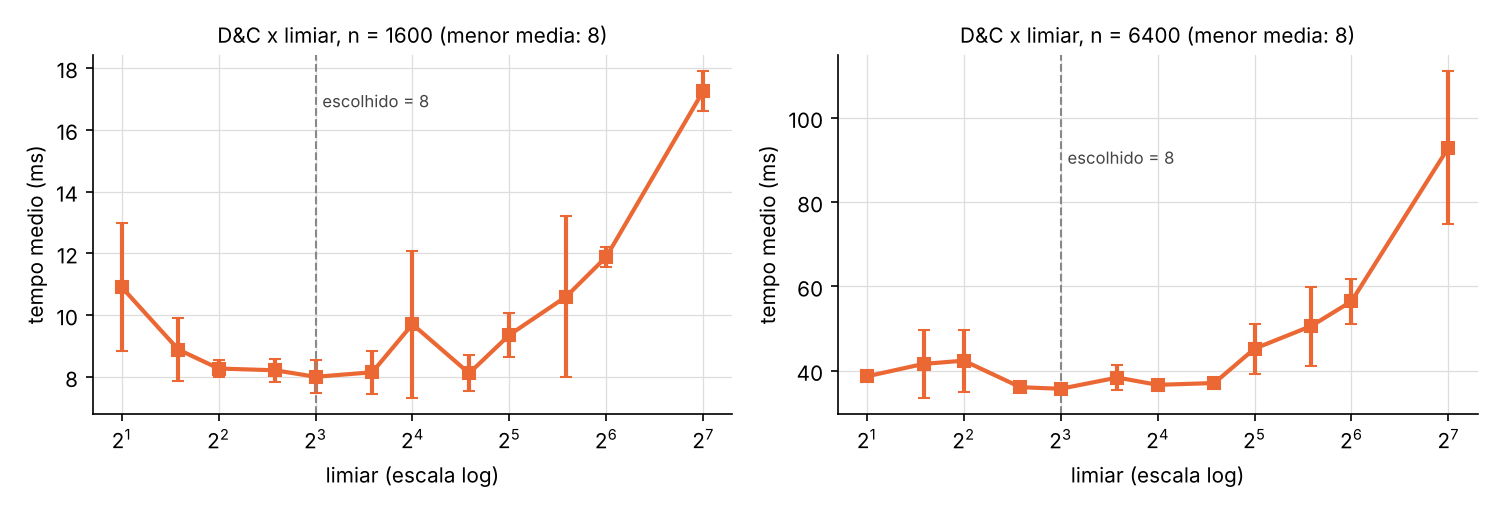
\includegraphics[width=\linewidth]{../resultados/etapa2_limiar.png}
\caption{Tempo médio da D\&C em função do limiar (barras = desvio padrão). A linha tracejada marca o valor escolhido.}\label{fig:lim}
\end{figure}

\begin{itemize}
  \item \textbf{Limiar grande demais ($L\ge32$):} o tempo sobe rápido. Com $L=128$ fica cerca de $2{,}2$ vezes maior (17,3 contra 8,0\,ms em $n=1600$) porque as folhas, de custo $\Theta(L^2)$, passam a dominar. É o termo $nL$ da análise.
  \item \textbf{Limiar pequeno demais ($L=2,3$):} a recursão vai até subproblemas de 2 ou 3 pontos, e o custo das chamadas é maior que as poucas comparações economizadas. Com $L=2$ e $n=1600$ o tempo foi 36\% maior que com $L=8$.
  \item \textbf{Entre 6 e 24} há um ``platô'' em que as diferenças ficam dentro do desvio padrão. $L=8$ teve a \textbf{menor média nos dois tamanhos} (8,00\,ms e 35,7\,ms) e baixa variação, por isso foi o escolhido. Ele também é coerente com a Tabela~\ref{tab:peq}: com até $\approx$16 pontos, a força bruta é claramente mais rápida que a D\&C pura.
\end{itemize}

Um detalhe ajuda a interpretar o gráfico: como a lista é sempre dividida ao meio, só importam os tamanhos que realmente aparecem na recursão. Com $n=6400$ os tamanhos são $6400, 3200, \dots, 50, 25, 12/13, 6/7$. Assim, $L=16$ e $L=24$ geram \emph{exatamente} a mesma árvore (folhas de 12 e 13 pontos), e a diferença medida entre eles (36,6 e 37,1\,ms) dá uma ideia do tamanho do ruído da medição.

\section{Conclusão}

As três implementações da Etapa~1 e as duas da Etapa~2 passaram em todos os testes, inclusive nos casos de borda e nas milhares de comparações aleatórias com a força bruta. As medições confirmaram as recorrências: $\Theta(n^2)$ para a força bruta, $\Theta(n\log n)$ para a D\&C ($T(n)=2T(n/2)+\Theta(n)$) e $\Theta(n)$ para o Kadane. Também ficou claro que a complexidade assintótica não conta a história toda. Para entradas pequenas ($n\lesssim32$) a força bruta é mais rápida, e é exatamente isso que justifica usar um limiar ($L=8$) na Etapa~2, aproveitando o melhor das duas abordagens.

\end{document}
